\documentclass{article}
\usepackage{graphicx}
\usepackage{adjustbox}
\usepackage{float}
\usepackage{geometry}

% Set custom page margins
\geometry{
	left=3cm,    % left margin
	right=3cm,   % right margin
	top=2.5cm,     % top margin
	bottom=2.5cm,  % bottom margin
}

\title{Vision-Based Lego Detection, Localization, and Assembly Using UR5 Robot Arm\\
\large Bachelor Thesis Project Report}
\author{Anh Tu Duong}
\date{\today}

\begin{document}
	
	\maketitle
	
	\section{Introduction}
	This progress report provides an overview of the work completed so far in the project "Vision-Based Lego Detection, Localization, and Assembly Using UR5 Robot Arm". The project aims to achieve autonomous pick-and-place assembly of Lego blocks using a UR5 robot arm.
	
	\begin{figure}[H]
		\centering
		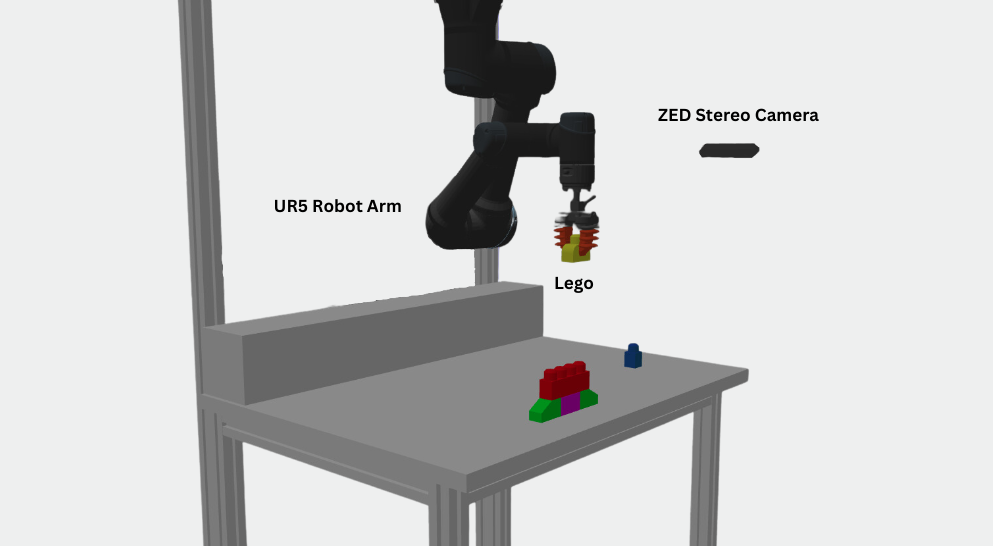
\includegraphics[width=0.75\textwidth]{images/scene-start.png}
		\caption{UR5 robot with ZED camera and Lego blocks on the table}
		\label{fig:scene-start}
	\end{figure}
	
	\section{Methodology}
	The methodology is structured around the implementation of three ROS (Robot Operating System) nodes representing the core components of the system:
	\begin{itemize}
		\item Vision: Responsible for object detection and localization. This node captures data from the ZED stereo camera, processes it using computer vision algorithms, and publishes relevant information on ROS topics.
		\item Motion: Dedicated to robot arm manipulation, including trajectory planning and control. This node subscribes to information from the Vision Node, determining optimal trajectories for the UR5 robot arm, and executing precise movements.
		\item Planning: Currently under development, this node will play a pivotal role in systematic task planning and coordination. Once fully implemented, it will communicate with both the Vision and Motion nodes, orchestrating the sequence of actions required for Lego construction.
	\end{itemize}
	
	\begin{figure}[H]
		\centering
		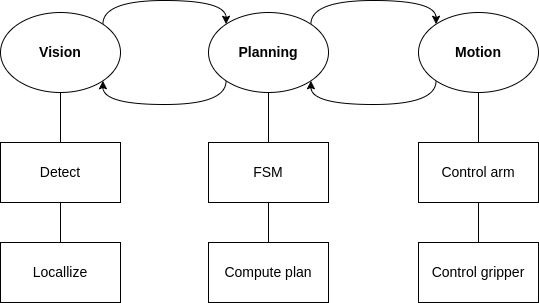
\includegraphics[width=0.6\textwidth]{images/design-main.png}
		\caption{Main workflow}
		\label{fig:design-main}
	\end{figure}
	
	\subsection{Vision}
	The Vision component serves as the perception module of the robot. The result we want to achieve is sending Lego's position and orientation to the robot.
	
	\begin{figure}[H]
		\centering
		\makebox[\textwidth][c]{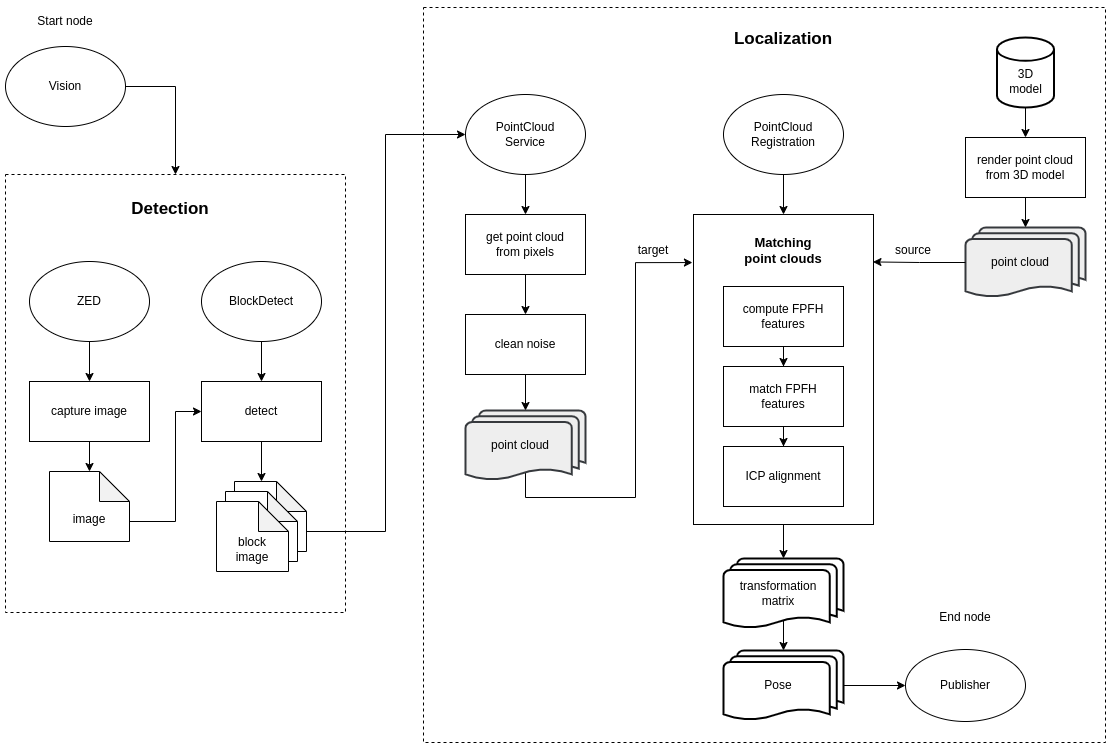
\includegraphics[width=1.2\textwidth]{images/design-vision.png}}
		\caption{Vision workflow}
		\label{fig:design-vision}
	\end{figure}
	
	\subsubsection{Detection}
	Detection is the first phase in the Vision workflow, aiming to identify and classify Lego blocks within the robot's field of view. In order to do that, a preprocess phase consisted of Dataset collection and Object detection model training has been done.
	
	\paragraph{Dataset collection}
	A dataset (about 14000 images) containing real images (10\%) from the ZED camera and synthetic images (90\%) generated from Blender with 3D models has been collected.
	
	\begin{figure}[H]
		\centering
		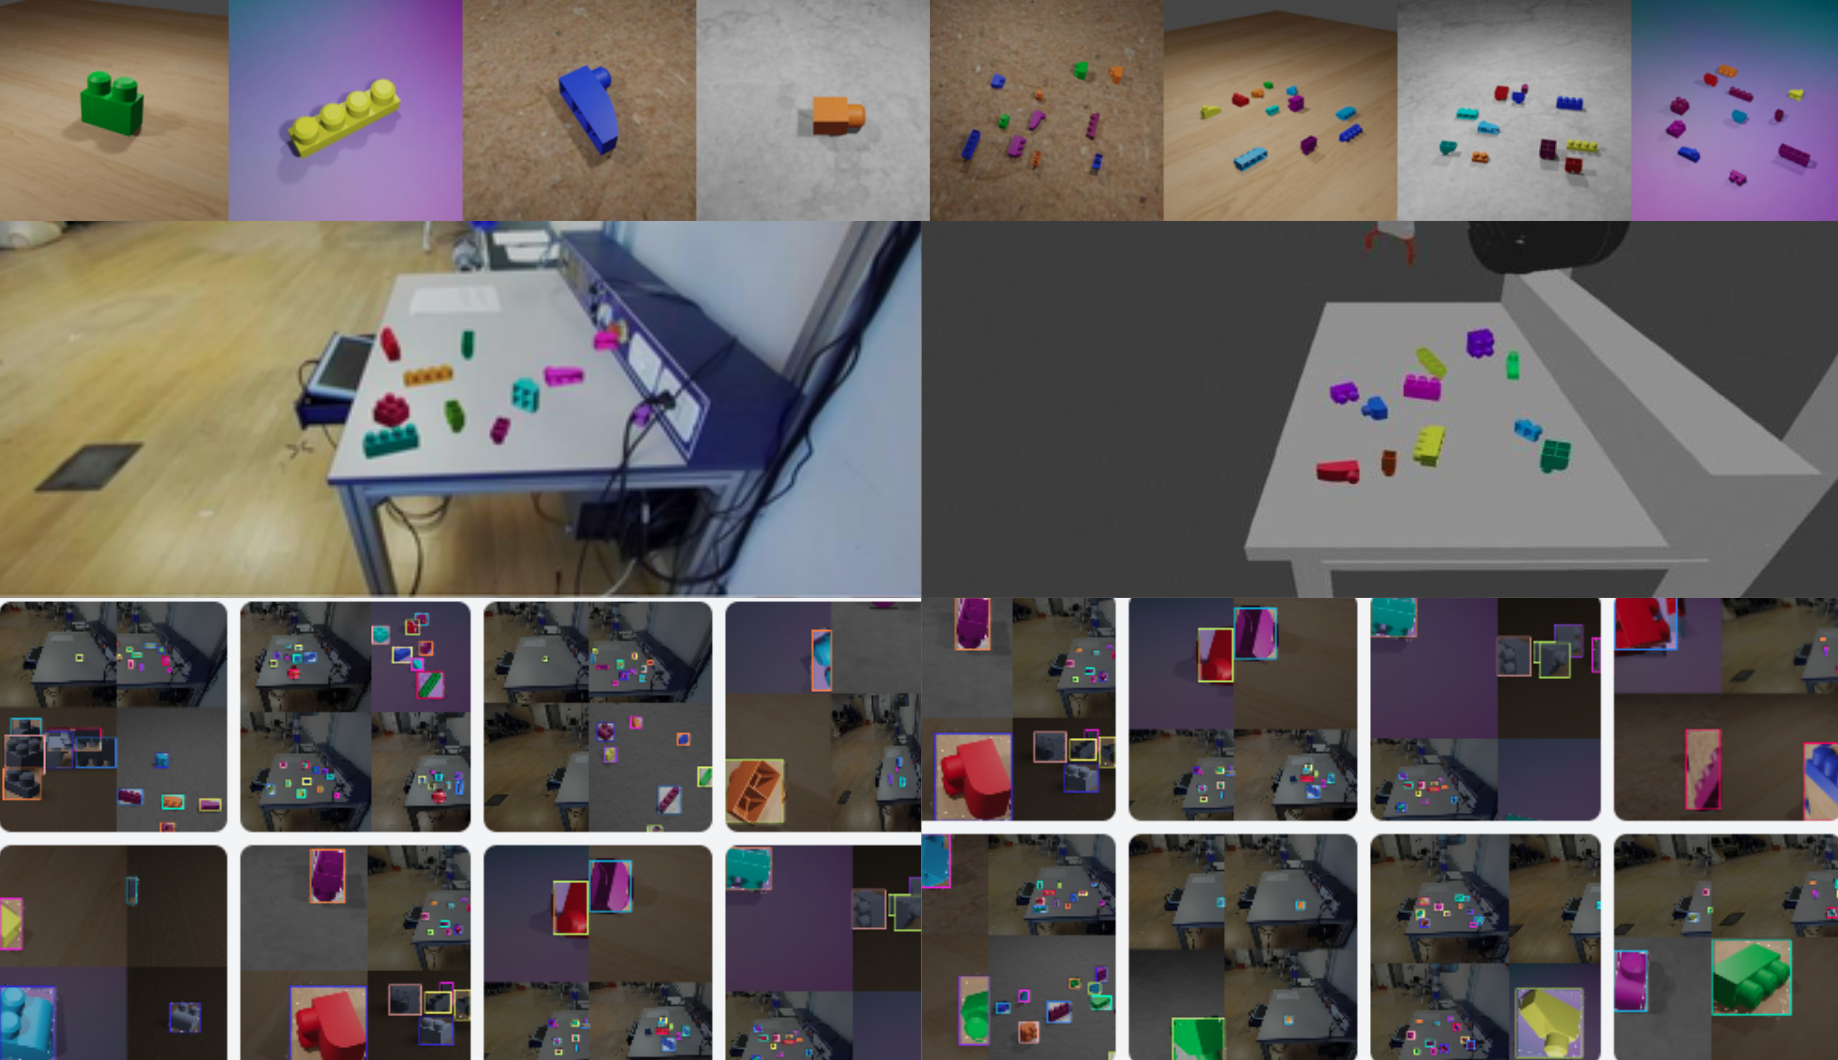
\includegraphics[width=1.0\textwidth]{images/dataset.png}
		\caption{Dataset}
		\label{fig:dataset}
	\end{figure}
	
	The dataset is divided into:
	\begin{itemize}
		\item Training set (86\%): 12000 images
		\item Validation set (11\%): 1600 images
		\item Testing set (3\%): 400 images
	\end{itemize}
	
	\paragraph{YOLO training}
	YOLOv8L was employed to train an object detection model. After 300 epochs, the model gets 98.5\% accuracy.
	
	\begin{figure}[H]
		\centering
		\makebox[\textwidth][c]{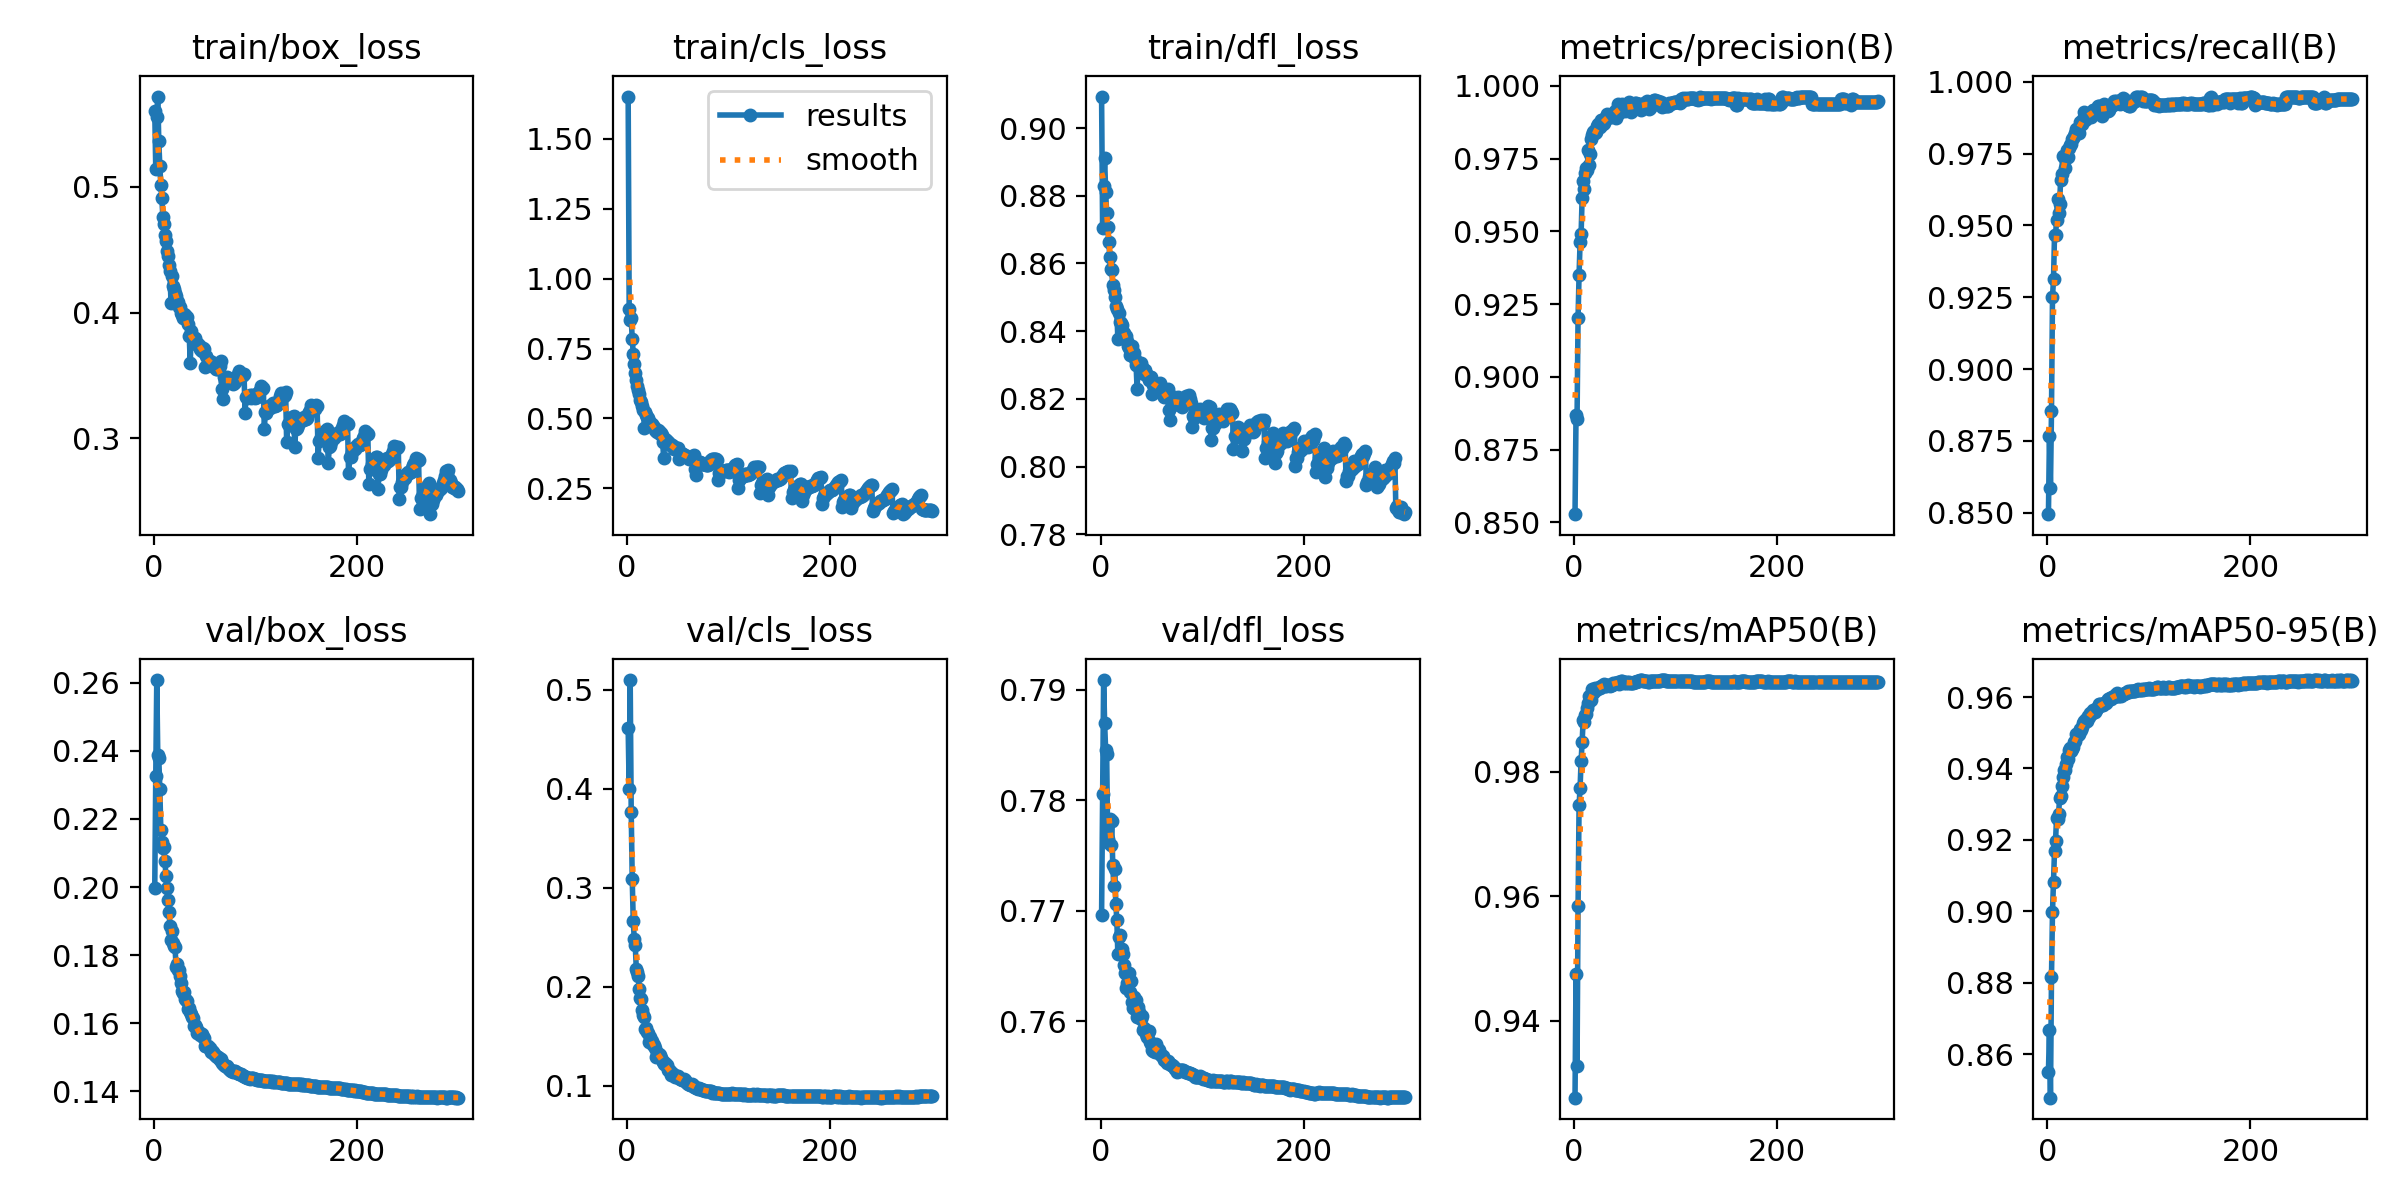
\includegraphics[width=1.1\textwidth]{images/yolo_train_results.png}}
		\caption{YOLOv8 train results}
		\label{fig:train_results}
	\end{figure}
	
	\begin{figure}[H]
		\centering
		\makebox[\textwidth][c]{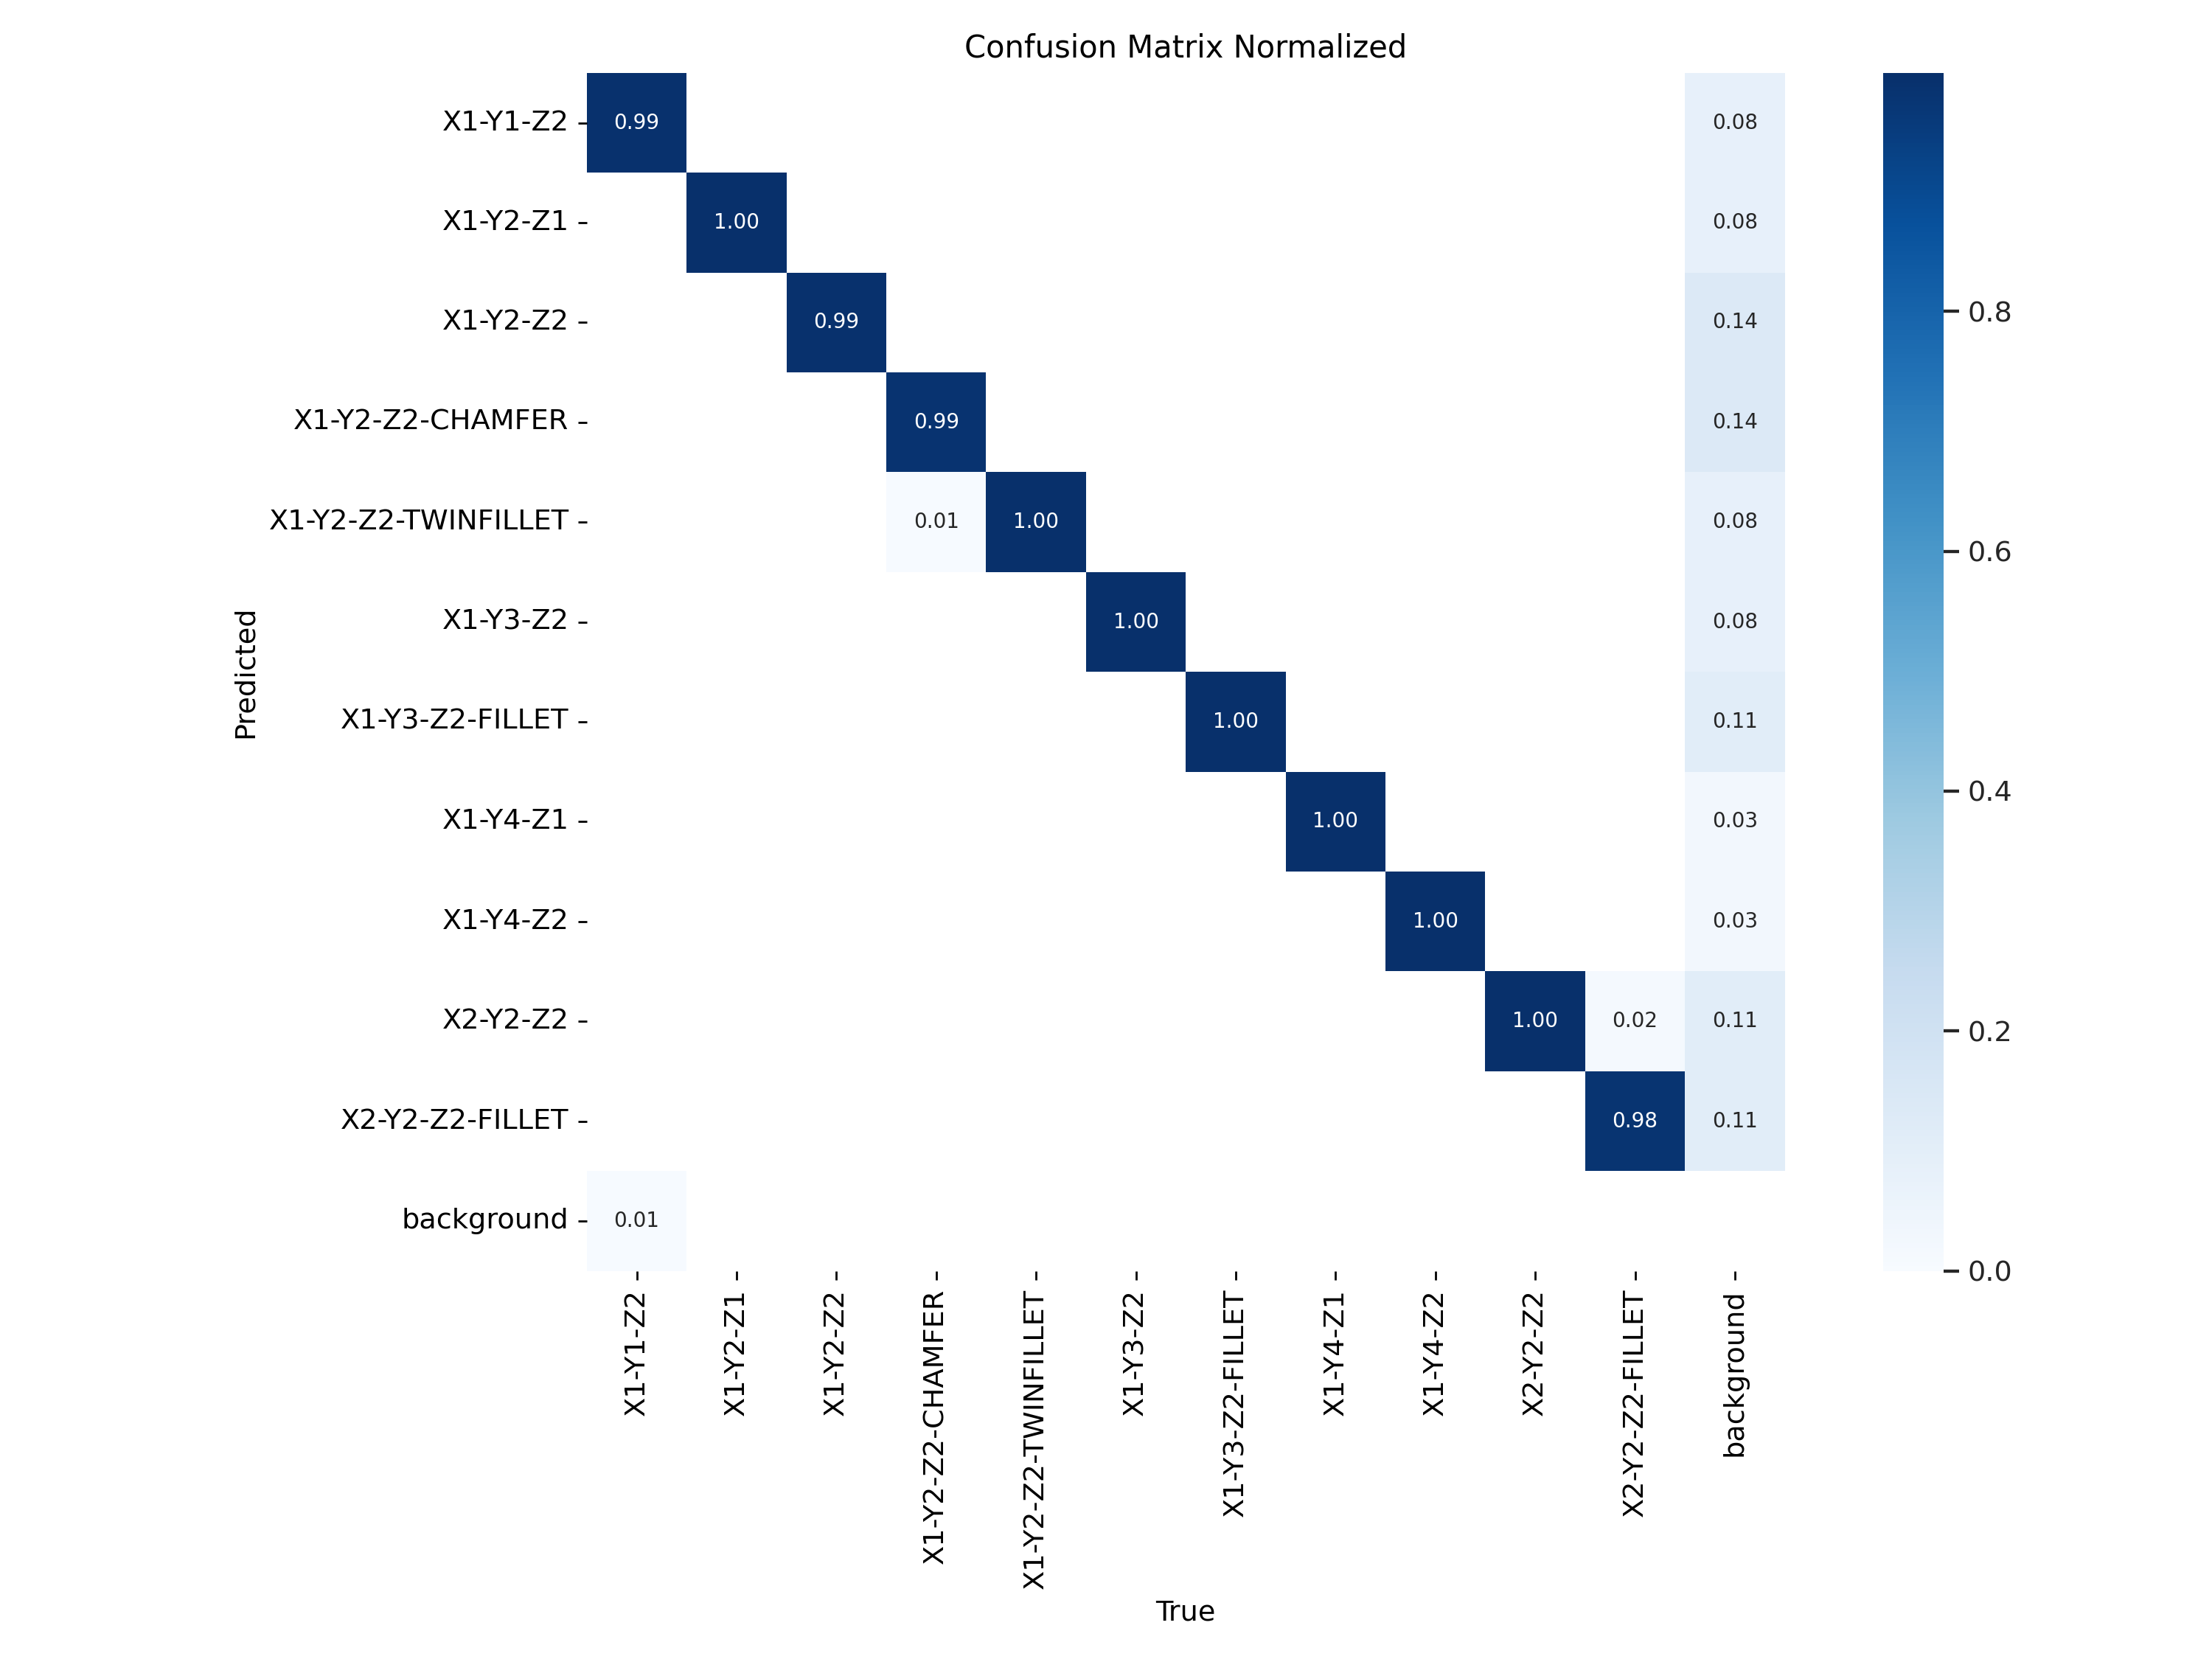
\includegraphics[width=1.0\textwidth]{images/confusion_matrix.png}}
		\caption{Confusion matrix}
		\label{fig:confusion_matrix}
	\end{figure}
	
	The Vision node starts with capturing images from the ZED camera and detecting Lego blocks using the trained YOLOv8 model. The bounding box information for detected objects is passed to the Localization process.
	
	\begin{figure}[H]
		\centering
		\makebox[\textwidth][c]{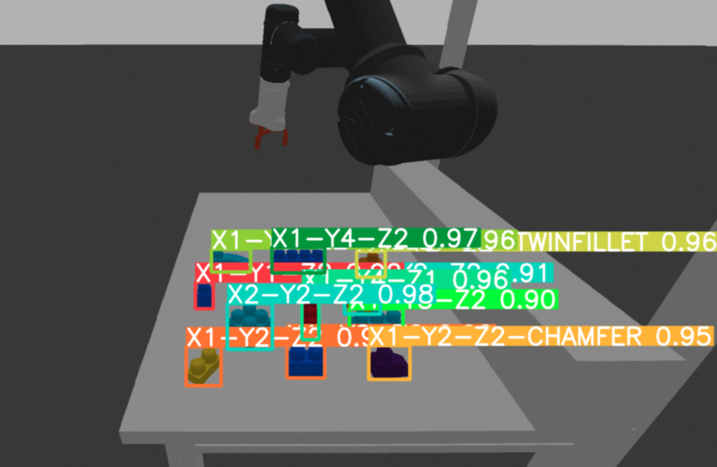
\includegraphics[width=0.8\textwidth]{images/detect.png}}
		\caption{Object detection using YOLOv8}
		\label{fig:detect}
	\end{figure}
	
	\subsubsection{Localization}
	The objective of Localization phase is to transform the initially detected 2D information of Lego blocks into a comprehensive 3D understanding. This crucial step bridges the gap between the robot's perception and its ability to interact with the physical world, enabling precise positioning and orientation of the objects within the three-dimensional workspace. The bounding boxes from the Vision component are used to extract point clouds of every pixels from the ZED camera data. After cleaning the point cloud belonging to the table, the rest represents a fragment of Lego blocks.
	
	\begin{figure}[H]
		\centering
		\makebox[\textwidth][c]{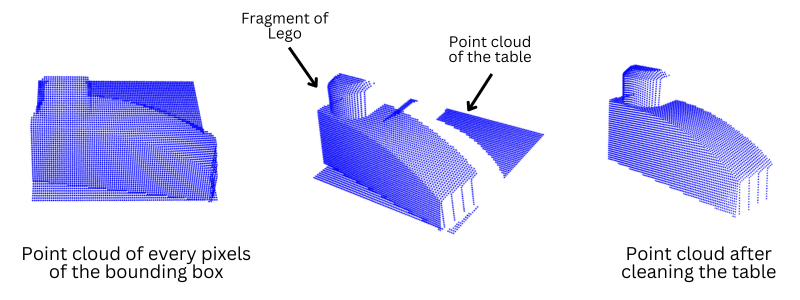
\includegraphics[width=0.8\textwidth]{images/pointcloud-clean.png}}
		\label{fig:pointcloud-clean}
	\end{figure}
	
	\paragraph{Point cloud generation from 3D Lego model}
	Point clouds were generated from the 3D models of the Lego blocks to represent their shapes. These point clouds will be matching with the point clouds of the Lego in the scene to localize it.
	
	\begin{figure}[H]
		\centering
		\makebox[\textwidth][c]{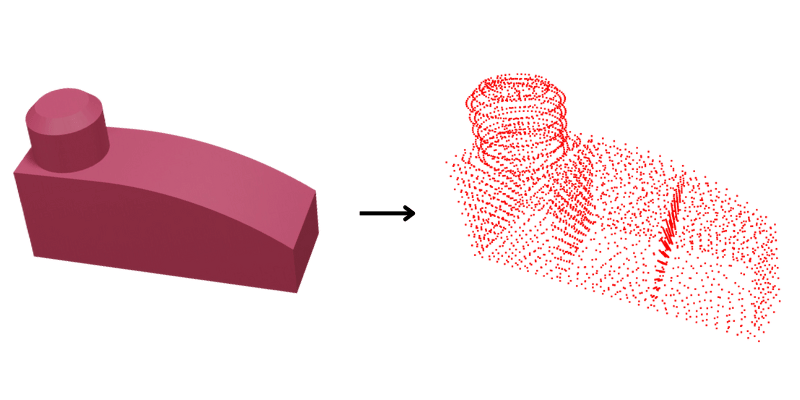
\includegraphics[width=0.5\textwidth]{images/pointcloud-from-3d.png}}
		\caption{From 3D Lego model to point cloud}
		\label{fig:pointcloud-from-3d}
	\end{figure}
	
	\paragraph{Point Cloud Registration}
	Point Cloud Registration is a fundamental problem in 3D computer vision and photogrammetry. Given several sets of points in different coordinate systems, the aim of registration is to find the transformation that best aligns all of them into a common coordinate system. Point Cloud Registration plays a significant role in this localization phase. Having point cloud rendered from the 3D model mesh (source point cloud) and the point cloud of an object detected from ZED camera (target point cloud), we need to perform some calculation to align the source point cloud to the target point cloud. The transformation matrix calculated after alignment is the pose of the Lego object in the scene.
	
	\begin{figure}[H]
		\centering
		\makebox[\textwidth][c]{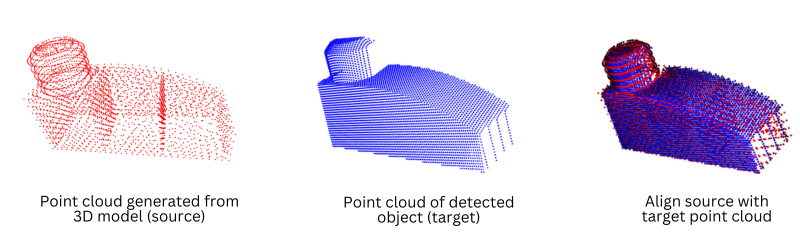
\includegraphics[width=0.9\textwidth]{images/pointcloud-align.png}}
		\caption{Point cloud registration}
		\label{fig:pointcloud-align}
	\end{figure}
	
	FPFH and ICP are 2 algorithms used to perform point cloud registration:
	
	\subparagraph{FPFH}
	
	FPFH (Fast Point Feature Histograms) is a feature descriptor commonly used in point cloud analysis and 3D computer vision tasks. It is an extension of the Point Feature Histograms (PFH) descriptor, designed to capture the geometric properties of 3D points. The FPFH descriptor calculates the local surface characteristics of a point in a point cloud by considering its neighbors. Here's a high-level overview of how FPFH features are computed:
	\begin{itemize}
		\item Select a point of interest (the query point) in the point cloud.
		\item Identify the k-nearest neighbors of the query point.
		\item For each neighbor, calculate the relative position with respect to the query point, forming a pairwise point-pair feature.
		\item Compute the difference in normal directions between the query point and each neighbor.
		\item Calculate a weighted histogram of the pairwise point-pair features, where the weights are based on the differences in normal directions.
		\item Concatenate the histograms from all the neighbors to obtain the final FPFH feature for the query point.
	\end{itemize}
	
	The FPFH descriptor takes into account not only the geometric positions of the neighboring points but also the differences in their surface normals. This combination allows for a more robust representation of local surface properties and provides a measure of distinctiveness between different points.
	
	\subparagraph{ICP}
	
	ICP stands for Iterative Closest Point. The ICP algorithm iteratively finds the best transformation that minimizes the distance between corresponding points in the two point clouds. The steps of ICP can be summarized as follows:
	\begin{itemize}
		\item Initialization: Define an initial transformation matrix that represents the rough alignment between the two point clouds. This initial transformation can be computed using some other method, or simply set to the identity matrix if no prior information is available.
		\item Correspondence: Find the corresponding points between the source point cloud and the target point cloud. One common method is to find the nearest neighbors in the target point cloud for each point in the source point cloud.
		\item Compute transformation: Compute the transformation that best aligns the corresponding points. One common method is to use Singular Value Decomposition (SVD) to compute the rotation and translation that minimize the sum of squared distances between corresponding points.
		\item Update transformation: Update the transformation matrix with the computed rotation and translation.
		\item Check convergence: Check if the convergence criterion is met. This can be done by comparing the change in the transformation matrix between iterations with a predefined threshold. If the convergence criterion is not met, go back to step 2 and repeat until convergence is reached.
		\item Output: The final transformation matrix gives the registration result. Apply this transformation to the source point cloud to align it with the target point cloud.
	\end{itemize}
	
	\subsection{Motion}
	The Motion component is responsible for trajectory planning and robot control.
	
	\begin{figure}[!ht]
		\centering
		\makebox[\textwidth][c]{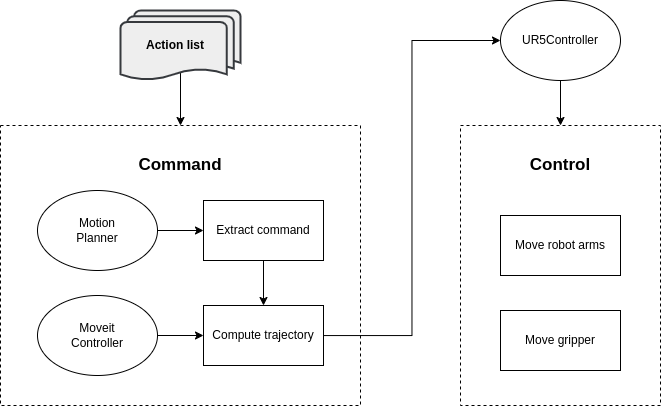
\includegraphics[width=0.8\textwidth]{images/design-motion.png}}
		\caption{Motion node workflow}
		\label{fig:design-motion}
	\end{figure}
	
	\subsubsection{Trajectory Planning}
	Has been developed with the help of the MoveIt package. MoveIt is a powerful motion planning framework in ROS that simplifies trajectory planning and robot arm manipulation. Using the target poses and orientations provided, MoveIt calculates feasible trajectories for the robot arm. These trajectories ensure safe and efficient pick-and-place movements, taking into account the robot's kinematics and workspace limitations.
	
	\subsubsection{Robot Control}
	With the trajectories determined, the Motion node sends control commands to the UR5 robot arm, enabling it to navigate to specified locations, grasp Lego blocks and accurately place them at the desired positions to construct the predefined structure.
	
	\subsection{Planning: (Work in Progress)}
	The Planning component is responsible for high-level task planning and error handling, integrating Vision and Motion nodes.
	
	\section{Challenge and Next Steps}
	To complete the project, the following steps need to be taken:
	
	\begin{itemize}
		\item \textbf{Develop the Planning Component:} The Planning component needs to be designed and implemented to coordinate the communication between the Vision and Motion nodes, generate a high-level plan for the robot arm, and handle error scenarios.
		\item \textbf{Construction image as input:} While the current construction process follows a pre-defined configuration (the final position of each Lego block is known), the next step involves incorporating the ability to interpret and process construction images as input. This enhancement aims to make the system more versatile, allowing it to adapt to variety of Lego constructions beyond the predefined configurations.
		\begin{figure}[!ht]
			\centering
			\makebox[\textwidth][c]{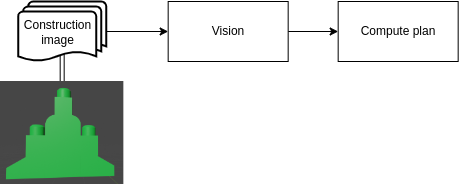
\includegraphics[width=0.7\textwidth]{images/design-image-as-input.png}}
			\caption{Image as input}
			\label{fig:input-image}
		\end{figure}
		\item \textbf{Refinement for vision accuracy:} The vision accuracy refinement step involves fine-tuning the algorithms responsible for detecting and localizing Lego blocks. This refinement ensures a higher level of precision in translating visual data into actionable information, reducing errors in the alignment of the point cloud.
		\begin{figure}[!ht]
			\centering
			\makebox[\textwidth][c]{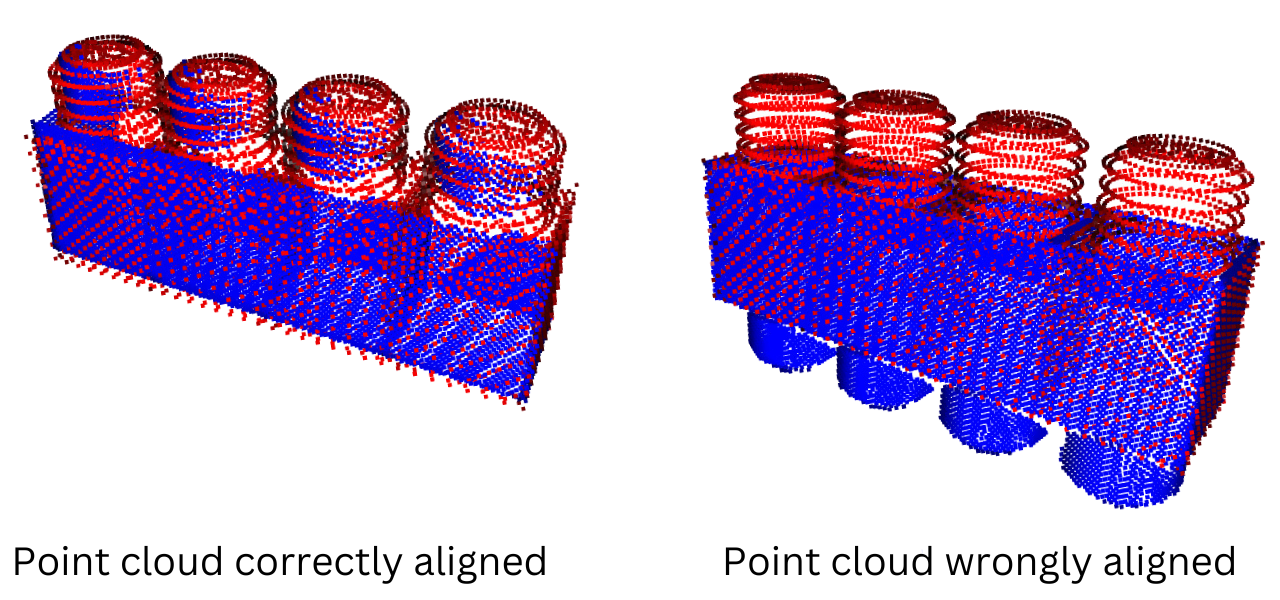
\includegraphics[width=0.6\textwidth]{images/pointcloud-wrong.png}}
			\caption{Point cloud registration}
			\label{fig:pointcloud-wrong}
		\end{figure}
	\end{itemize}
	
	\section{Conclusion}
	The "Vision-Based Lego Detection, Localization, and Assembly Using UR5 Robot Arm" project has made significant progress in implementing the Vision and Motion components. However, the Planning component remains to be developed, which poses the primary challenge. Addressing the difficulties in planning and implementing robust error handling will be crucial to achieving a fully autonomous Lego block assembly system. With further development and refinement, the project has the potential to demonstrate the capabilities of vision-based robotics in real-world applications.
	
\end{document}
